\section{Implementasi Kakas Konversi}

Pada bagian ini, penulis membahas poin-poin penting dan spesifikasi implementasi kakas.
Tugas akhir ini membahas alur-alur implementasi yang penting, mulai dari bagaimana konfigurasi dibaca, bagaimana pembangkitan dan penggabungan kode dilakukan, serta hal-hal lain yang dilakukan oleh kakas ini.
Struktur kode dari implementasi penulis juga akan dibahas pada bagian ini.

\subsection{Spesifikasi Umum Kakas}

Kakas ini diimplementasikan pada bahasa pemrograman Go.
Hal ini dilakukan karena rata-rata kakas untuk banyak hal diimplementasikan untuk bahasa Go yang \textit{executable}-nya cukup kecil.
Selain itu, bahasa Go merupakan bahasa yang \textit{strongly typed}, sehingga dapat memudahkan perbaikan atau penambahan fitur ke depannya.
Walaupun Python adalah bahasa yang umum digunakan dalam eksperimen pemelajaran mesin, kakas ini tidak terkait dengan penggunaan kakas-kakas yang spesifik hanya ada di Python saja, sehingga penggunaan bahasa lain tidak menjadi masalah.

Kakas ini akan menghasilkan kode Python yang siap dijalankan.
Kode juga mencakup file-file lain yang diperlukan.
Kode yang dihasilkan akan menggunakan \textit{framework} seperti \monospace{FastAPI} yang merupakan \textit{framework} aplikasi web yang umum digunakan.
Alasan pengunaan FastAPI adalah karena selain umum digunakan, \textit{framework} ini menghasilkan kode yang cukup sederhana dan mudah dipahami.

Kakas ini diuji dalam sistem berbasis kernel Linux.
Walau begitu, dengan implementasi dan bahasa Go yang digunakan seharusnya kakas ini dapat digunakan dalam lingkungan sistem yang berbeda.
Untuk menggunakan kakas ini, Python juga diperlukan untuk melakukan instalasi \textit{library} yang diperlukan agar sistem dapat berjalan.
\textit{Library} yang diinstalasi akan disiapkan dalam sebuah \textit{virtual environment}.

\subsection{Struktur Direktori Kakas}

Bagian ini akan menjelaskan mengenai struktur direktori dari kakas yang dibuat.
Tujuan bagian ini adalah untuk memahami struktur kode yang dibuat penulis dalam mengembangkan kakas serta menambahkan fungsionalitas kepada kakas.
Untuk rincian dari implementasi kode \url{https://github.com/mkamadeus/myx}.

\begin{figure}[ht]
    \vspace{\baselineskip}
    \centering
    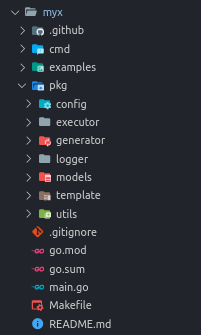
\includegraphics[width=0.4\textwidth]{resources/images/chapter-4/04-directory.png}
    \caption{Struktur Direktori Kakas}\label{fig:04-directory}
\end{figure}

Gambar~\ref{fig:04-directory} menunjukkan bagaimana struktur direktori dari kakas.
Masing-masing direktori dalam kakas ini bertanggung jawab untuk suatu hal.
Berikut adalah penjelasan singkat masing-masing direktori yang ada.

\begin{enumerate}
    \item Direktori \monospace{cmd}

    Direktori ini merupakan \textit{``main''} dari kakas.
    Kakas yang menggunakan \textit{library} \monospace{cobra} menggunakan direktori ini untuk mengeksekusi satuan pekerjaan yang ada dalam kakas.
    Untuk implementasi kakas ini saat ini hanya diimplementasikan untuk menghasilkan kode.

    \item Direktori \monospace{pkg/config}
    
    Direktori ini bertanggung jawab atas konfigurasi dari kakas ketika dijalankan.
    Konfigurasi yang diatur seperti apakah kakas akan mengeluarkan \textit{log} yang rinci dan mengatur di mana lokasi spesifikasi sistem berada.

    \item Direktori \monospace{pkg/executor}
    
    Direktori ini bertanggung jawab untuk melakukan eksekusi terhadap \textit{shell} tempat kakas ini dijalankan.
    Utamanya, \textit{executor} yang berada dalam kakas ini berfungsi untuk melakukan instalasi \textit{library} Python melalui pip.

    \item Direktori \monospace{pkg/generator}
    
    Direktori ini merupakan direktori yang digunakan untuk menyimpan \textit{generator} penghasil kode.
    Kode sistem akan digabungkan pada direktori ini; bergantung pada format masukan yang diinginkan untuk sistem.

    \item Direktori \monospace{pkg/logger}
    
    Direktori ini menyimpan \textit{instance logger} untuk kakas ini.
    Kakas ini menggunakan \textit{library} \monospace{logrus} untuk melakukan \textit{logging}.

    \item Direktori \monospace{pkg/models}
    
    Direktori ini memodelkan model-model data yang diperlukan untuk kakas ini.
    Salah satu model data yang disimpan dalam direktori ini adalah konfigurasi kakas yang akan dibaca dari YAML.\@
    Selain itu, direktori ini juga dapat menyimpan pemetaan tipe data antara konfigurasi kakas ke tipe data dalam kode.

    \item Direktori \monospace{pkg/template}
    
    Direktori ini menyimpan dan menghasilkan potongan kode dalam bentuk \textit{template}.
    Potongan kode yang disimpan disimpan dalam \textit{file} terpisah yang nantinya akan digunakan dalam kakas menggunakan bantuan \textit{library} Go bawaan yaitu \monospace{embed}.
    Potongan kode yang disimpan dibagai ke beberapa subdirektori untuk masing-masing jenis kode.
    Secara rata-rata, kode dibangun untuk bisa diimplementasikan secara independen, tetapi terdapat sebuah pengecualian untuk direktori \monospace{pkg/template/pipeline}.

    Direktori \monospace{pkg/template/pipeline} mendefinisikan modul-modul pemrosesan data yang ada.
    Modul-modul ini berupa potongan kode yang bila digabungkan akan membentuk satu kesatuan pemrosesan data.
    Oleh karena itu, \textit{template} dari modul ini perlu dipertimbangkan, apakah diimplementasikan secara independen atau tidak.
    Rincian mengenai modul akan dibahas pada Bagian~\ref{section:04-module}.

    \item Direktori \monospace{pkg/utils}
    
    Direktori ini adalah direktori yang menyimpan fungsi dan prosedur bantuan yang digunakan dalam seluruh program.
    Fungsi dan prosedur bantuan tersebut meliputi operasi yang meliputi \textit{string} waktu itu.
    
\end{enumerate}


\subsection{Pembacaan Konfigurasi}

Sesuai yang telah dibahas pada bagian sebelumnya, masing-masing bagian konfigurasi bertanggung jawab atas suatu bagian dalam kode.
Konfigurasi mengatur juga alur pembangkitan kode dilakukan.
Gambar~\ref{fig:04-flowchart-config-read} menunjukan alur pembacaan konfigurasi oleh kakas hingga terbentuknya kode sistem.

\begin{figure}[ht]
  \vspace{\baselineskip}
    \centering
    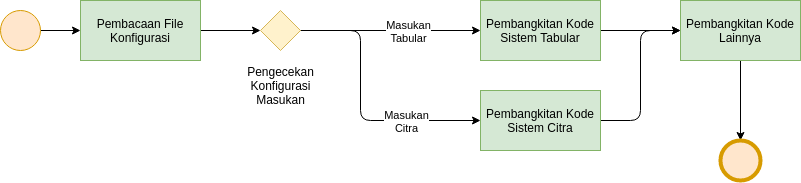
\includegraphics[width=\textwidth]{04-alur-pembacaan-konfigurasi.drawio.png}
    \caption{Alur Pembacaan Konfigurasi oleh Kakas}\label{fig:04-flowchart-config-read}
\end{figure}

Berdasarkan bagian sebelumnya, kakas memodelkan konfigurasi secara internal; artinya tipe dari kakas akan diperiksa ketika kakas akan di-\textit{compile} dan dalam \textit{runtime}.
Masing-masing bagian konfigurasi dimodelkan secara terpisah untuk tiap bagian dari konfigurasi.
Konfigurasi juga didefinisikan seumum mungkin agar mudah untuk melakukan penambahan fungsionalitas kakas secara mudah.


\subsection{Pembangkitan dan Penggabungan Kode}

\begin{figure}[ht]
  \vspace{\baselineskip}
    \centering
    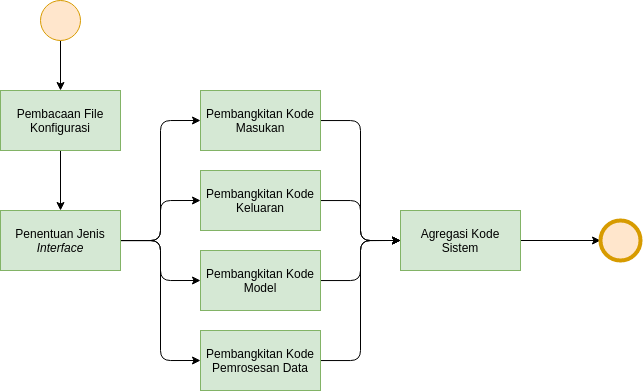
\includegraphics[width=\textwidth]{04-alur-pembangkitan-umum.drawio.png}
    \caption{Alur Pembangkitan oleh Kakas}\label{fig:04-flowchart-code-generation}
\end{figure}

Secara umum, pembangkitan kode dilakukan dalam beberapa tahap seperti yang dideskripsikan pada Gambar~\ref{fig:04-flowchart-code-generation}, yaitu sebagai berikut:
\begin{enumerate}
    \item Penentuan jenis \textit{interface}
    \item Pembangkitan kode masukan
    \item Pembangkitan kode keluaran
    \item Pembangkitan kode model
    \item Pembangkitan kode pemrosesan data
    \item Agregasi kode
\end{enumerate}

Keseluruhan proses pembangkitan kode ini dilakukan melalui penerimaan masukan yang diperlukan untuk masing-masing bagian kode.
Kemudian, dengan masukan serta \textit{template} untuk bagian kode tersebut dapat dibangkitkan sepotong kode.
Sepotong kode akan dikembalikan oleh fungsi dan disimpan untuk digabungkan. 

Bagian sebelumnya telah membahas lebih detail tentang bagaimana bagian-bagian konfigurasi bertanggung jawab terhadap bagian kode dan keterkaitannya dengan masing-masing kode.
Bila disederhanakan, kelima tahapan tersebut dapat mencakup seluruh proses pembangkitan kode.
Akibat dibangkitkan secara terpisah, diperlukan tahapan tambahan untuk menggabungkan kode.

Agregasi kode pada dasarnya menggunakan implementasi yang serupa pada pembangkitan bagian-bagian kode, yaitu menerima masukan nilai-nilai yang diperlukan; dalam hal ini adalah kode yang telah dibangkitkan, serta \textit{template} yang membentuk kode utama sistem.
Segala hal yang berkaitan bagaimana \textit{framework} yang dipilih dibangun berada dalam tahapan ini.
\textit{Endpoint} didefinisikan dalam tahapan ini.
Sebuah \textit{endpoint} dibangun dari potongan-potongan kode yang telah dibangun sebelumnya.

Dalam tahapan agregasi kode, terdapat suatu tahapan yang menggabungkan definisi \textit{import} yang diperlukan dari berbagai bagian kode.
Suatu tahapan diperlukan untuk melakukan analisis kode untuk melakukan instalasi \textit{library} yang diperlukan.

\subsection{Pembangkitan File Terkait}

Selain dari membangkitkan kode, diperlukan beberapa \textit{file} lagi untuk memastikan sistem ini dapat berjalan.
Beberapa file yang penulis tetapkan untuk dibuat adalah seperti berikut:

\begin{enumerate}
    \item \textit{File} Dockerfile; dibuat agar sistem bisa dijalankan melalui \textit{container}.
    \item \textit{File} Gitignore; dibuat untuk memudahkan pengguna bila kode akan dimasukkan ke dalam \textit{version control system}.
    \item \textit{File library} Python/\monospace{requirements.txt}; dibuat agar diketahui apa saja kakas-kakas yang diperlukan.
\end{enumerate}

Secara umum, pembangkitan \textit{file-file} ini dilakukan oleh penulis dengan mekanisme yang sederhana untuk kakas ini.
Dibuat \textit{template} dari \textit{file-file} yang diperlukan yang akan dibaca oleh kakas dan dibangkitkan setelah semua proses sebelumnya selesai.
Bila diperlukan, dapat didefinisikan kode tambahan untuk melakukan penambahan \textit{file}.

Pengecualian untuk \textit{file library} Python \monospace{requirements.txt}; \textit{file} ini akan dihasilkan oleh kakas ketika melakukan instalasi \textit{library} yang diperlukan.
Kakas akan melakukan analisis terhadap \textit{library-library} yang diperlukan berdasarkan \textit{import} yang dilakukan.
Kakas kemudian akan mengunduh \textit{library} yang bersesuaian.
Setelah semua \textit{library} berhasil diinstalasi, \textit{file} \monospace{requirements.txt} ini akan dibuat.

\subsection{Modul Pemrosesan Data}\label{section:04-module}

Dalam kakas ini, sudah terbuat beberapa modul pemrosesan data untuk pemrosesan yang umum digunakan.
Contoh modul pemrosesan data yang sudah ada seperti melakukan \textit{terhadap} data tabular, melakukan \textit{resizing} terhadap data citra, dan ada beberapa modul lainnya.
Definisi modul dalam kakas ini adalah kumpulan \textit{template} kode yang modular yang bila digabungkan menjadi satu akan membentuk kesatuan kode yang menghasilkan data yang dapat diterima oleh model.

Struktur suatu modul dalam kakas dapat direpresentasikan dalam beberapa hal seperti berikut:
\begin{enumerate}
    \item \textit{Template} kode
    \item Nilai masukan untuk \textit{template}
    \item Nama unik untuk modul
\end{enumerate}

\textit{Template} kode untuk modul merupakan kode Python yang dirancang sedemikian sehingga bila kode-kode tersebut diisi dengan nilai masukan yang bersesuaian untuk \textit{template} tersebut, akan menghasilkan alur pemrosesan data yang runtut.
Bergantung dari jenis masukannya, urutan modul pada konfigurasi akan berpengaruh pada hasil akhir kode.
Misalnya untuk data tabular, urutan tidak begitu menjadi perhatian karena biasanya akan dilakukan pemrosesan per kolom (kecuali untuk pemrosesan yang perlu dilakukan secara terurut).

Nama unik untuk modul saat ini dikodekan secara langsung di dalam kakas, sehingga perlu didefinisikan sebuah nama yang unik dalam kakas.
Kakas akan mencocokan nama yang ada dalam konfigurasi untuk membuat masukan \textit{template} yang akan dibuat menjadi kode sesungguhnya.
Dalam implementasi kakas ini, karena modul dibuat berada dalam kakas, perlu dilakukan perubahan terhadap kakas untuk menambah modul.

Berdasarkan hal-hal yang membentuk sebuah modul, pengguna dapat membuat modul baru bila diinginkan untuk kasus yang akan diuji.
Penambahan modul baru dapat dilakukan melalui menambah ketiga hal tersebut di dalam kode.
Untuk rinciannya, dapat dilihat pada kode kakas untuk melihat kode program yang perlu ditambah atau diubah.
